% This is a sample LaTeX input file.  (Version of 12 August 2004.)
%
% A '%' character causes TeX to ignore all remaining text on the line,
% and is used for comments like this one.

\documentclass{article}      % Specifies the document class

                             % The preamble begins here.
\title{\bf Principles of Computer Systems Design\\ {\Large Assignment 2}}  % Declares the document's title.
\author{Tudor Dragan\\
Gabriel Carp}      % Declares the author's name.
\date{December 2, 2014}      % Deleting this command produces today's date.

\usepackage{verbatimbox}
\usepackage{listings}
\usepackage{color}
\usepackage[]{amsmath}
\usepackage[english]{babel}
\usepackage[utf8]{inputenc}
\usepackage{graphicx}
\usepackage{moreverb}
\usepackage{hyperref}
\usepackage[T1]{fontenc} % font
\usepackage{program}
\usepackage[top=1.5in, bottom=1.5in, left=1.4in, right=1.4in]{geometry}
\usepackage[super]{nth}

\definecolor{dkgreen}{rgb}{0,0.6,0}
\definecolor{gray}{rgb}{0.5,0.5,0.5}
\definecolor{mauve}{rgb}{0.58,0,0.82}

\lstset{frame=tb,
      language=Java,
      aboveskip=3mm,
      belowskip=3mm,
      showstringspaces=false,
      columns=flexible,
      basicstyle={\small\ttfamily},
      numbers=none,
      numberstyle=\tiny\color{gray},
      keywordstyle=\color{blue},
      commentstyle=\color{dkgreen},
      stringstyle=\color{mauve},
      breakatwhitespace=true
      tabsize=3
}
\newcommand{\ip}[2]{(#1, #2)}
                             % Defines \ip{arg1}{arg2} to mean
                             % (arg1, arg2).

%\newcommand{\ip}[2]{\langle #1 | #2\rangle}
                             % This is an alternative definition of
                             % \ip that is commented out.

\begin{document}             % End of preamble and beginning of text.

\maketitle                   % Produces the title.

\section*{Question 1: Serializability \& Locking} 

Conflict-serializability is defined by equivalence to a serial schedule (no overlapping transactions) with the same transactions, such that both schedules have the same sets of respective chronologically ordered pairs of conflicting operations (same precedence relations of respective conflicting operations).\\

A schedule is conflict-serializable if and only if it's precedence graph has no cycles. This is a graph of nodes and vertices, where the nodes are the transaction names and the vertices are attribute collisions.\\

\subsection*{Schedule 1}

Schedule 1 \emph{is not} conflict serializable because the graph is \emph{cyclic}:
\begin{itemize}
\item $T_1$ - $T_2$: read-write conflict on $X$.
\item $T_2$ - $T_3$: write-read conflict on $Z$.
\item $T_3$ - $T_1$: read-write conflict on $Y$.
\end{itemize}

\subsection*{Schedule 2}

Schedule 2 \emph{is} conflict serializable because the precedence graph is \emph{acyclic}:
\begin{itemize}
\item $T_1$ - $T_2$: $X$ is accessed by $T_2$ after $T_1$ has committed.
\item $T_2$: $Y$ is only accessed by $T_2$.
\item $T_3$ - $T_2$: $Z$ exclusively locked by $T_3$ is released prior to $T_2$ acquiring a
shared lock.
\end{itemize}

\section*{Question 2: Optimistic Concurrency Control}

\subsection*{Scenario 1}

Because $T_1$ finishes before $T_3$ starts, the \nth{1} condition holds. We have to check that the \nth{2} condition holds for $T_2$ and $T_3$, but because $T_2$ writes the object that $T_3$ reads from, this condition does not hold. Therefore $T_3$ has to \emph{rollback}.\\

\subsection*{Scenario 2}

The \nth{2} validation condition does not hold for $T_1$ and $T_3$ because $T_1$ writes to object 3 and $T_3$ reads from it. Therefore $T_3$ has to rollback. We can observe that the \nth{3} holds for $T_2$, because $T_3$ does not access object 8.\\

\subsection*{Scenario 3}

The only object that $T_1$ writes to is object 4 and because $T_3$ does not read or write to that object, the \nth{2} validation condition holds. Then we check is the \nth{2} condition holds for $T_2$ and $T_3$. $T_2$ only writes to object 6 and $T_3$ does not access that object in any way, therefore $T_3$ can commit.\\

\section*{Programming Task}

For the implementation of the locking protocol used in the ConcurrentCertainBookStore we used the \emph{ReentrantReadWriteLock} class available in the \emph{java.util.concurrent.locks} package. \\

A ReentrantLock is owned by the thread last successfully locking, but not yet unlocking it. A thread invoking lock will return, successfully acquiring the lock, when the lock is not owned by another thread. The method will return immediately if the current thread already owns the lock.\\

The ReentrantReadWriteLock allows both readers and writers to reacquire read or write locks in the style of a ReentrantLock. Non-reentrant readers are not allowed until all write locks held by the writing thread have been released. Additionally, a writer can acquire the read lock, but not vice-versa. Among other applications, reentrancy can be useful when write locks are held during calls or callbacks to methods that perform reads under read locks. If a reader tries to acquire the write lock it will never succeed.\\

We implemented the strict two-phase locking (S2PL) by requiring a write lock when modifying the data at the start of the method. Some methods only require read locks such as getBooks and getBooksInDemand.\\

% Please add the following required packages to your document preamble:
% \usepackage[table,xcdraw]{xcolor}
% If you use beamer only pass "xcolor=table" option, i.e. \documentclass[xcolor=table]{beamer}
\begin{table}[h]
\begin{center}
\begin{tabular}{|c|c|c|}
\hline
{\bf{Lock type}} & \bf{read-lock} & \bf{write-lock} \\ \hline
\bf{read-lock} & \multicolumn{1}{l|}{} & \bf{X} \\ \hline
\bf{write-lock} & \bf{X} & \bf{X} \\ \hline
\end{tabular}
\caption{Lock compatibility table}
\label{Lock compatibility table}
\end{center}
\end{table}

\subsection*{Discussion on the Concurrent Implementation of Bookstore}

\subsubsection*{Is your locking protocol correct? Why? Argue for the correctness of your protocol by equivalence to a variant of 2PL.}

Our protocol is implemented by using the conservative S2PL by acquiring a lock at the beginning of each method and releasing it before the method returns.\\

\subsubsection*{Can your locking protocol lead to deadlocks? Explain why or why not.}

The deadlock cannot occur because we acquire the locks right at the start of the methods, transforming every call into an \emph{atomic} one. This approach impacts the performance by lowering concurrency, but ultimately assures proper synchronization.\\

\subsubsection*{Is/are there any scalability bottleneck/s with respect to the number of clients in the bookstore after your implementation? If so, where is/are the bottleneck/s and why? If not, why can we infinitely scale the number of clients accessing this service?}

Scalability is a problem because \emph{we lock the entire datastore} when we are modifying the database. We have taken into account the difference between readers and writers and we allow for multiple reads but not for multiple writes. A solution to this problem would be the fact that we acquire writing locks on the table entry level. For example, if a client modifies the stock of a book in the book store, we should not wait for the stock update when adding a rating.\\

\subsubsection*{Discuss the overhead being paid in the locking protocol in the implementation vs. the degree of concurrency you expect your protocol to achieve.}

It is safe to assume that the overhead is not that big. Because we are dealing with a bookstore, the customers that \emph{get and read}  more information about the books are more frequent, compared to the buyers that \emph{modify and change} the bookstore's stock and ratings. Our locking protocol is suitable enough for providing adequate isolation and performance.

\newpage
\appendix
\section*{\\Appendix 1: Serializability \& Locking}
% the \\ insures the section title is centered below the phrase: AppendixA

\begin{figure}[ht!]
\centering
 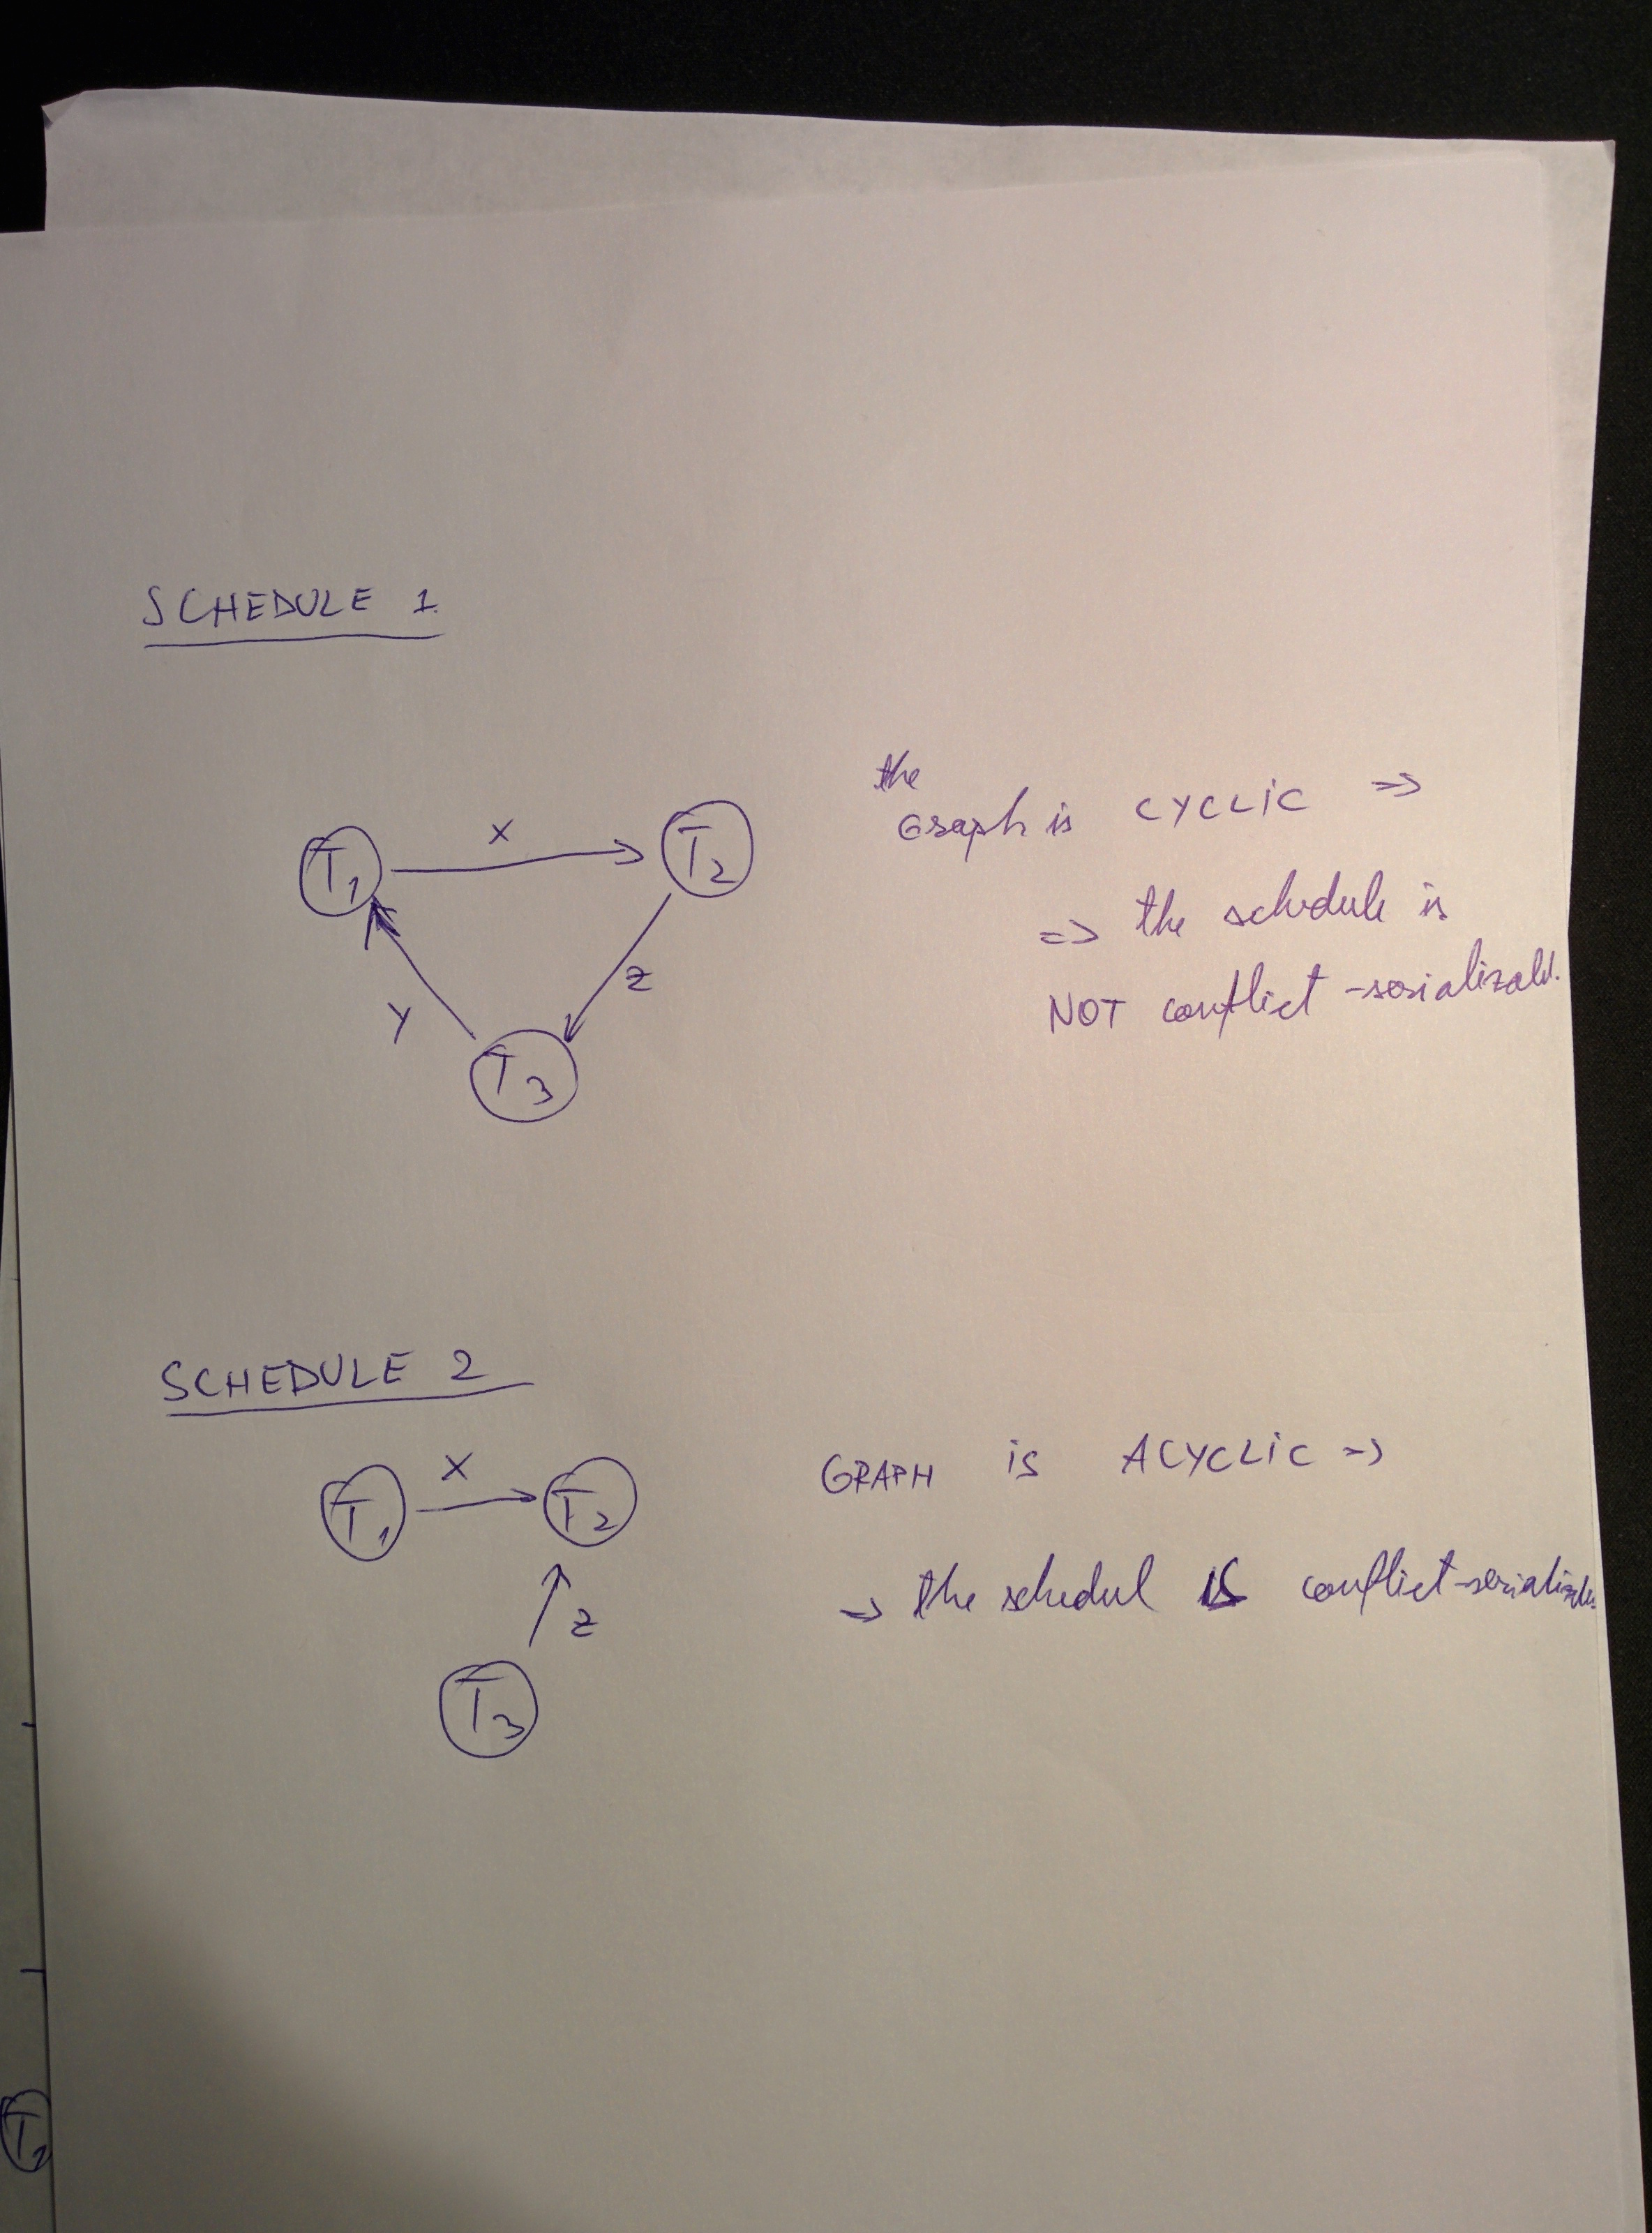
\includegraphics[scale=.15]{q1}
\caption{The precedence graphs for the two schedules \label{overflow}}
\end{figure}


\newpage
\section*{\\Appendix 2: Optimistic Concurrency Control}
% the \\ insures the section title is centered below the phrase: Appendix B
\begin{figure}[ht!]
\centering
 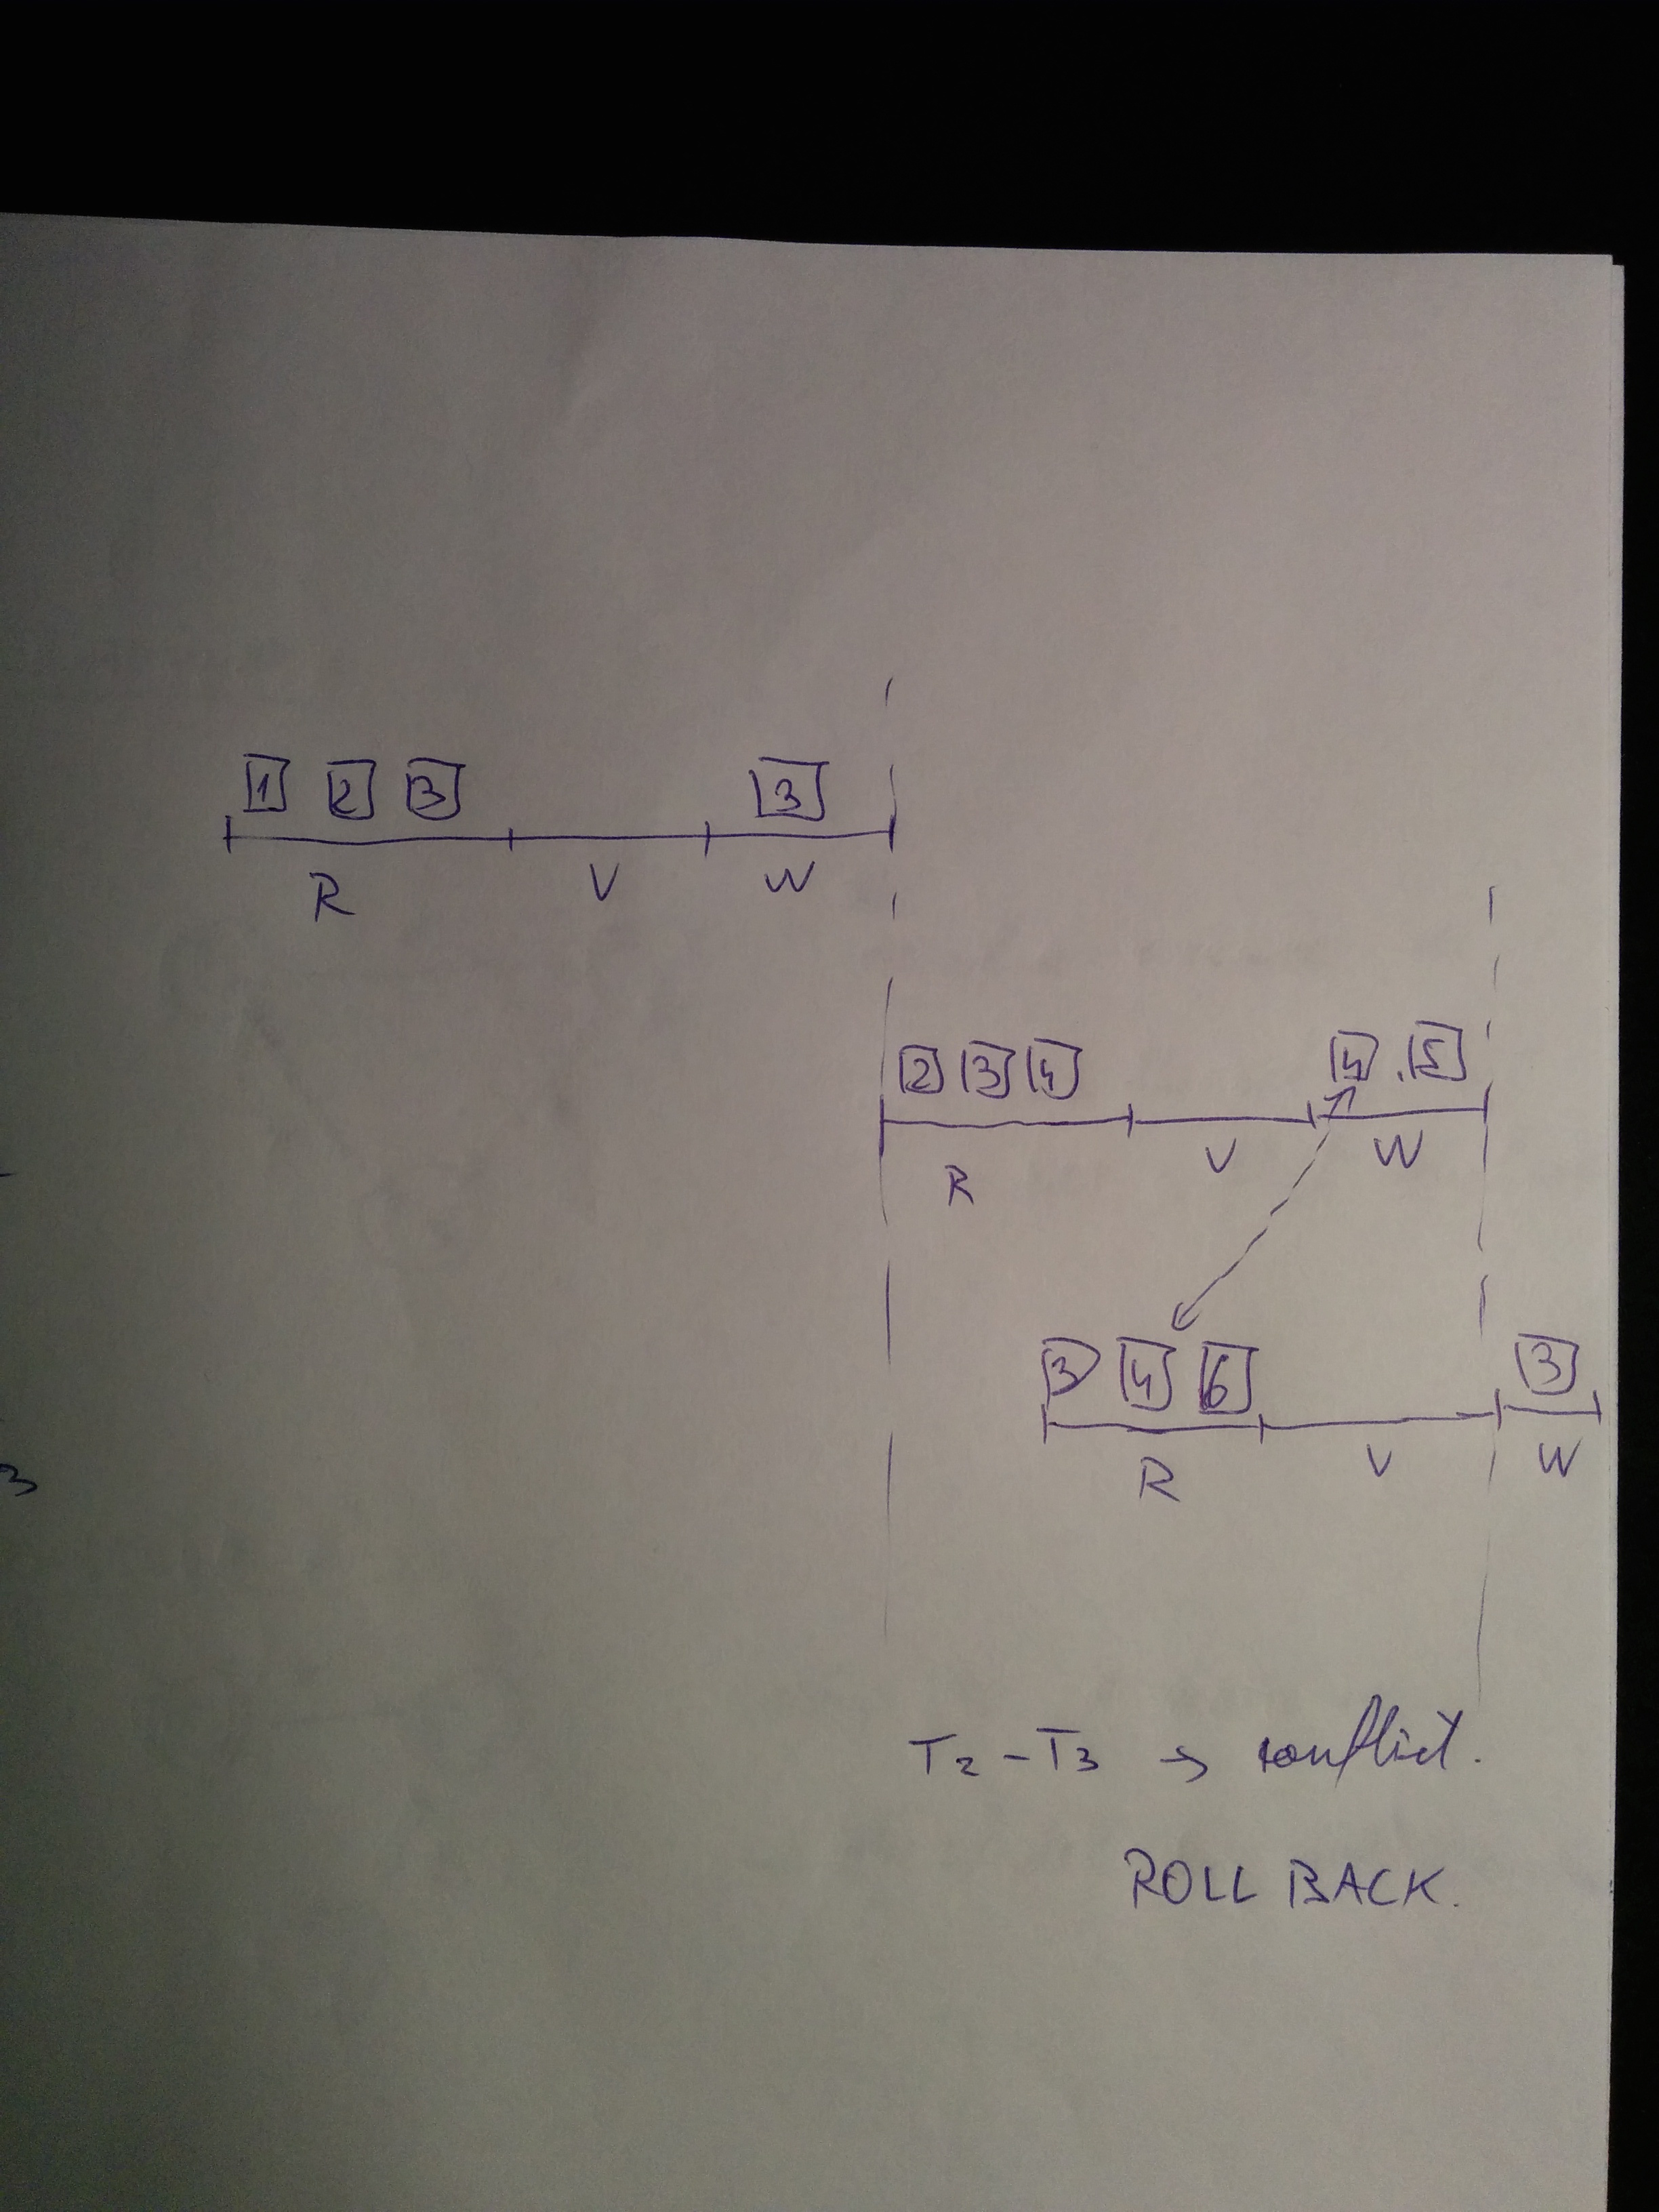
\includegraphics[scale=.15]{q2-1}
\caption{Scenario 1 \label{overflow}}
\end{figure}

\newpage

\begin{figure}[ht!]
\centering
 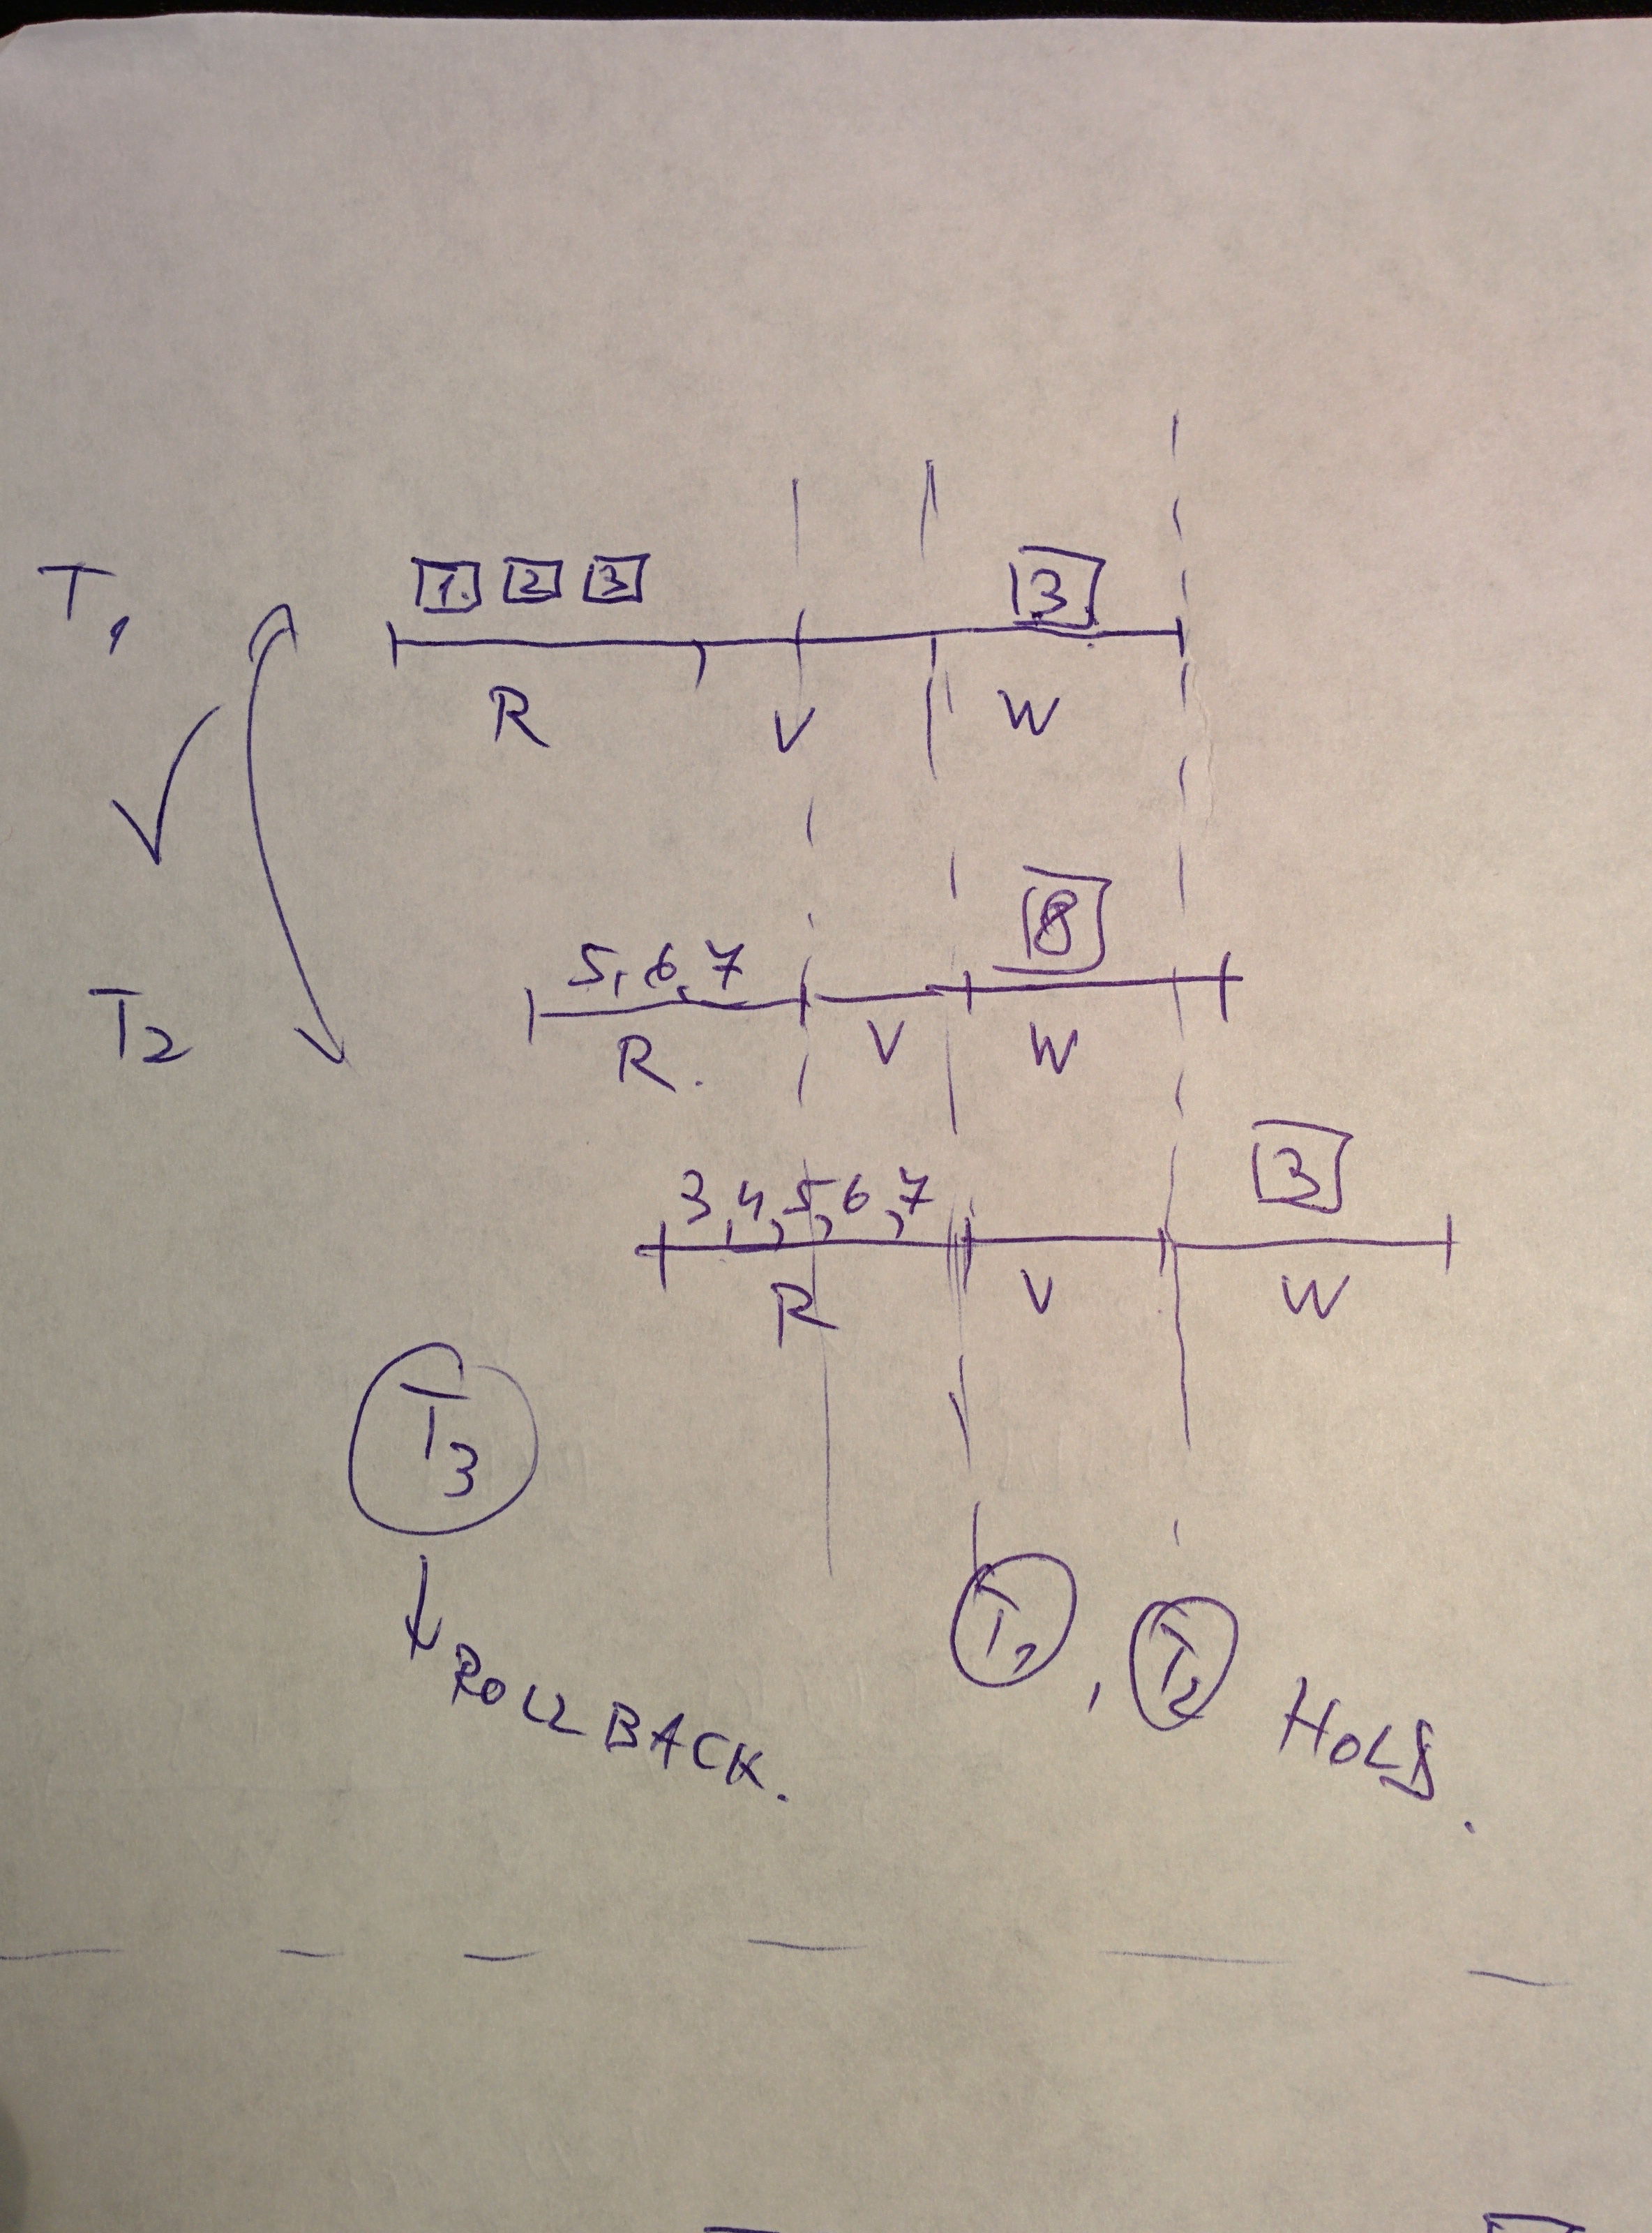
\includegraphics[scale=.15]{q2-2}
\caption{Scenario 2 \label{overflow}}
\end{figure}

 \newpage
\begin{figure}[ht!]
\centering
 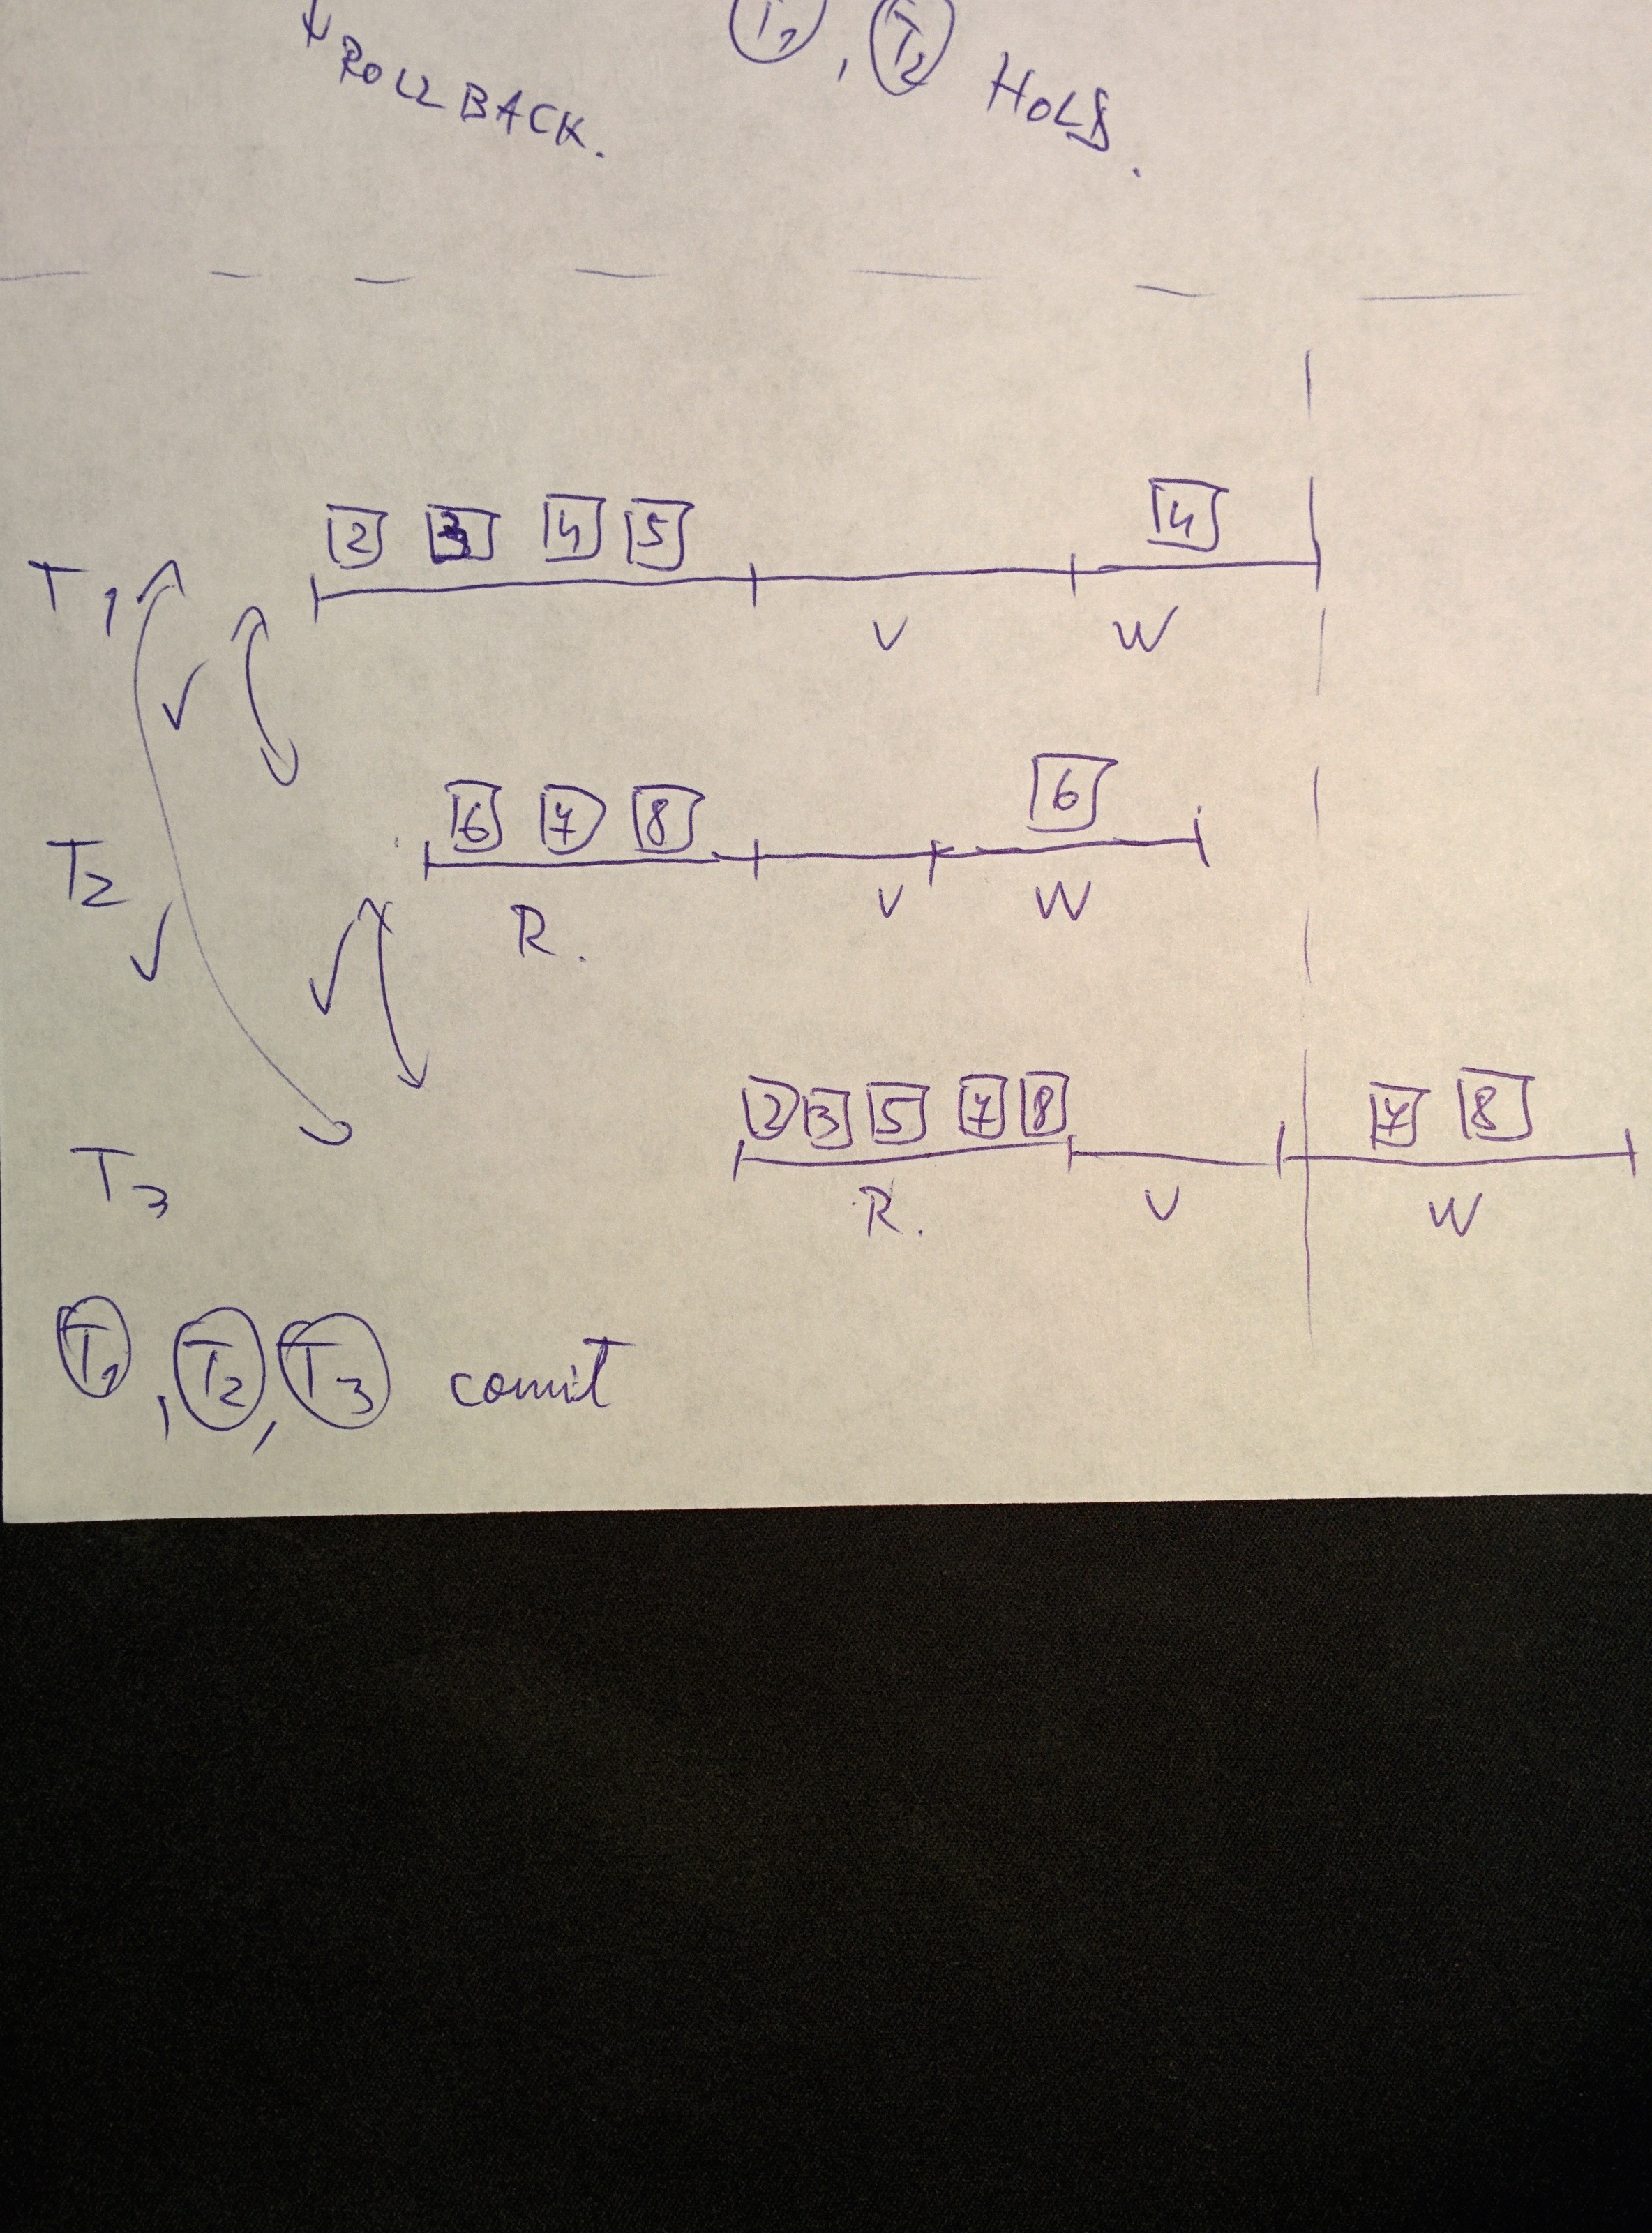
\includegraphics[scale=.15]{q2-3}
\caption{Scenario 3 \label{overflow}}
\end{figure}

\newpage

\end{document}               % End of document.